\iftoggle{title}{
\subsection*{Problem 2}
}{}
\iftoggle{contributions}{
\textit{Created by Tyler Wilson 2023}
}{}

\iftoggle{difficulty}{
Difficulty: $\medblackstar \medblackstar \medblackstar$
}{}

An insulating cylinder of radius $R$ and effectively infinite length in the z-direction contains a uniform charge density of $\rho$.
\begin{center}
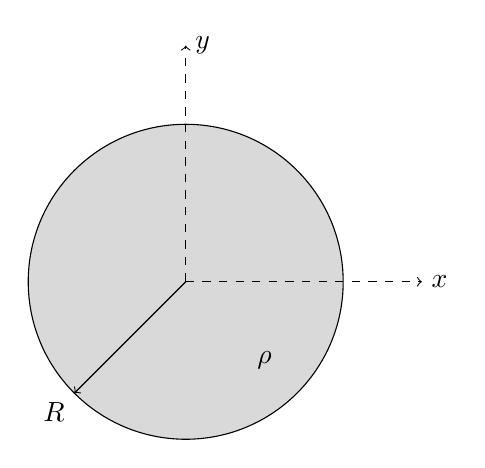
\begin{tikzpicture}
    \draw[fill=gray!30] (0,0) circle (2);
    \draw[dashed, ->] (0,0) -- (3,0) node[right] {$x$};
    \draw[dashed, ->] (0,0) -- (0,3) node[right] {$y$};
    \draw[->] (0,0) -- (-1.414,-1.414) node[below left] {$R$};
    \node at (1,-1) {$\rho$};
\end{tikzpicture}
\end{center}
\begin{enumerate}
    \item Find the electric field everywhere in space
\end{enumerate}
If there is now a \underline{hollow} spherical cavity of radius $a$ located at the center of the cylinder,
\begin{center}
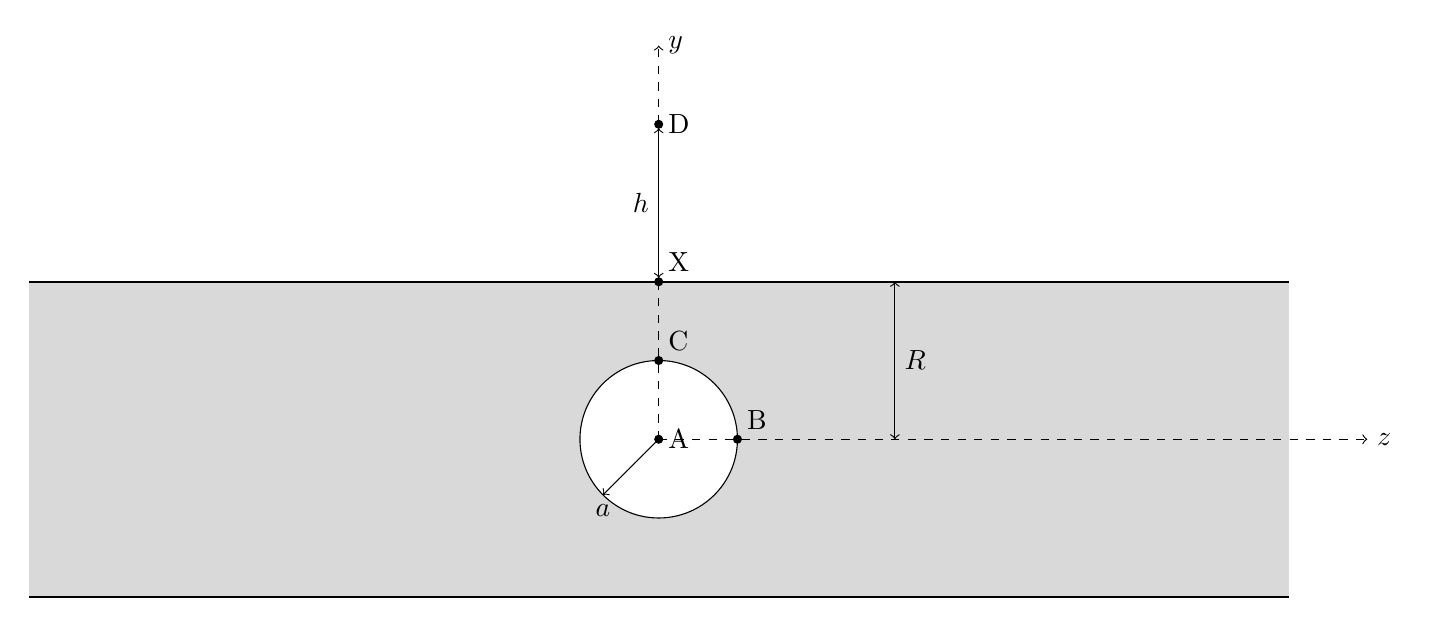
\begin{tikzpicture}
    \fill[gray!30] (-8,2) rectangle (8,-2);
    \draw[thick] (-8,2) -- (8,2);
    \draw[thick] (-8,-2) -- (8,-2);
    \draw[fill=white] (0,0) circle (1);
    \draw[fill=black] (0,0) circle (0.05) node[right] {A};
    \draw[fill=black] (1,0) circle (0.05) node[above right] {B};
    \draw[fill=black] (0,1) circle (0.05) node[above right] {C};
    \draw[fill=black] (0,4) circle (0.05) node[right] {D};
    \draw[fill=black] (0,2) circle (0.05) node[above right] {X};
    \draw[<->] (0,2.05) -- (0,3.95) node[midway, left] {$h$};
    \draw[->] (0,0) -- (-0.707,-0.707) node[below] {$a$};
    \draw[dashed, ->] (0,0) -- (0,5) node[right] {$y$};
    \draw[dashed, ->] (0,0) -- (9,0) node[right] {$z$};
    \draw[<->] (3,0) -- (3,2) node[midway, right] {$R$};
\end{tikzpicture}
\end{center}
\begin{enumerate}
    \setcounter{enumi}{1}
    \item Find the electric field at the center of the sphere at point A.
    \item Find the electric field just outside the sphere at point B.
    \item Find the electric field just outside the sphere at point C.
    \item Find the electric field outside both objects at point D.
\end{enumerate}
If the potential at the point X is 0V,
\begin{enumerate}
    \setcounter{enumi}{5}
    \item What is the potential at point A?
\end{enumerate}

\iftoggle{solutions}{
\textbf{Solution:}\\
\textit{Notation:} Because we have two types of radii, the cylindrical radius, and the spherical radius, we will use $s$ to represent the variable cylindrical radius and $r$ to represent the variable spherical radius.
\begin{enumerate}
\item We can use Gauss's Law to find the electric field everywhere in space. We will use a Gaussian cylinder of radius $s$ and length $L$.
\begin{align*}
    &\oiint\vec{E}\cdot d\vec{A}=\frac{Q_\text{enc}}{\epsilon_0}
\end{align*}
We will need to break this into two parts: the inside of the cylinder and the outside of the cylinder.\\
For the inside of the cylinder,
\begin{align*}
    &\oiint\vec{E}_\text{in}\cdot d\vec{A}=E_\text{in}A=\frac{Q_\text{enc}}{\epsilon_0}\\
    &Q_\text{enc}=\rho V_\text{enc}=\rho\pi s^2L\\
    &E_\text{in}A=\frac{\rho\pi s^2L}{\epsilon_0}\\
    &2\pi rLE_\text{in}=\frac{\rho\pi s^2L}{\epsilon_0}\\
    &E_\text{in}=\frac{\rho s}{2\epsilon_0}\\
    &\answer{\vec{E}_\text{in}=\frac{\rho s}{2\epsilon_0}\hat{s}}
\end{align*}
For the outside of the cylinder,
\begin{align*}
    &\oiint\vec{E}_\text{out}\cdot d\vec{A}=E_\text{out}A=\frac{Q_\text{enc}}{\epsilon_0}\\
    &Q_\text{enc}=\rho V_\text{enc}=\rho\pi R^2L\\
    &E_\text{out}A=\frac{\rho\pi R^2L}{\epsilon_0}\\
    &2\pi sLE_\text{out}=\frac{\rho\pi R^2L}{\epsilon_0}\\
    &E_\text{out}=\frac{\rho R^2}{2\epsilon_0s}\\
    &\answer{\vec{E}_\text{out}=\frac{\rho R^2}{2\epsilon_0s}\hat{s}}
\end{align*}
\item We can use the principle of superposition to find the electric field at point A. We will need to find the electric field due to the cylinder and the electric field due to the cavity and add the two together to get the total contribution.\\
The electric field due to the cylinder is given by
\[\vec{E}_\text{cyl}=\frac{\rho s}{2\epsilon_0}\hat{s}\eval_{s=0}=\vec{0}\]
To find the electric field from the cavity we can treat the cavity like a sphere of radius $a$ with a uniform charge density of $-\rho$. The electric field from this sphere can be computed using Gauss's Law.
\begin{align*}
    &\oiint\vec{E}\cdot d\vec{A}=EA=\frac{Q_\text{enc}}{\epsilon_0}
\end{align*}
We will also need to break this into two parts: the inside of the sphere and the outside of the sphere.\\
For the inside of the sphere,
\begin{align*}
    &Q_\text{enc}=-\rho V_\text{enc}=-\rho\frac{4}{3}\pi r^3\\
    &E_\text{in}A=E_\text{in}(4\pi r^2)=-\frac{\rho\frac{4}{3}\pi r^3}{\epsilon_0}\\
    &E_\text{in}=-\frac{\rho r}{3\epsilon_0}\\
    &\vec{E}_\text{in}=E_\text{in}\hat{r}=-\frac{\rho r}{3\epsilon_0}\hat{r}
\end{align*}
For the outside of the sphere,
\begin{align*}
    &Q_\text{enc}=-\rho V_\text{enc}=-\rho\frac{4}{3}\pi a^3\\
    &E_\text{out}A=E_\text{out}(4\pi r^2)=-\frac{\rho\frac{4}{3}\pi a^3}{\epsilon_0}\\
    &E_\text{out}=-\frac{\rho a^3}{3\epsilon_0r^2}\\
    &\vec{E}_\text{out}=E_\text{out}\hat{r}=-\frac{\rho a^3}{3\epsilon_0r^2}\hat{r}
\end{align*}
At point A, the electric field from the cavity will be
\[\vec{E}=-\frac{\rho r}{3\epsilon_0}\hat{r}\eval_{r=0}=\vec{0}\]
So the total electric field at point A is
\[\answer{\vec{E}_A=\vec{0}}\]
\item We will once again use superposition and can reuse the electric field from the cavity that we found in part (b) adn the cylinder in part (a). The electric field from the cylinder is given by
\[\vec{E}_\text{cyl,B}=\frac{\rho s}{2\epsilon_0}\hat{s}\eval_{s=0}=\vec{0}\]
The electric field from the cavity is given by
\[\vec{E}_\text{cav,B}=-\frac{\rho r}{3\epsilon_0}\hat{i}\eval_{r=a}=-\frac{\rho a}{3\epsilon_0}\hat{i}\]
So the total electric field at point B is
\[\answer{\vec{E}_B=-\frac{\rho a}{3\epsilon_0}\hat{i}}\]
\item For point C,\\
The electric field from the cylinder is given by
\[\vec{E}_\text{cyl,C}=\frac{\rho s}{2\epsilon_0}\hat{j}\eval_{s=a}=\frac{\rho a}{2\epsilon_0}\hat{j}\]
The electric field from the cavity is given by
\[\vec{E}_\text{cav,C}=-\frac{\rho r}{3\epsilon_0}\hat{j}\eval_{r=a}=-\frac{\rho a}{3\epsilon_0}\hat{j}\]
So the total electric field at point C is
\begin{align*}
    &\vec{E}_C=\vec{E}_\text{cyl,C}+\vec{E}_\text{cav,C}\\
    &\vec{E}_C=\frac{\rho a}{2\epsilon_0}\hat{j}-\frac{\rho a}{3\epsilon_0}\hat{j}\\
    &\answer{\vec{E}_C=\frac{\rho a}{6\epsilon_0}\hat{j}}
\end{align*}
\item For point D,\\
The electric field from the cylinder is given by
\[\vec{E}_\text{cyl,D}=\frac{\rho R^2}{2\epsilon_0s}\hat{j}\eval_{s=R+h}=\frac{\rho R^2}{2\epsilon_0(R+h)}\hat{j}\]
The electric field from the cavity is given by
\[\vec{E}_\text{cav,D}=-\frac{\rho r}{3\epsilon_0}\hat{j}\eval_{r=R+h}=-\frac{\rho (R+h)}{3\epsilon_0}\hat{j}\]
So the total electric field at point D is
\begin{align*}
    &\vec{E}_D=\vec{E}_\text{cyl,D}+\vec{E}_\text{cav,D}\\
    &\vec{E}_D=\frac{\rho R^2}{2\epsilon_0(R+h)}\hat{j}-\frac{\rho (R+h)}{3\epsilon_0}\hat{j}\\
    &\answer{\vec{E}_D=\frac{3\rho R^2-2\rho(R+h)^2}{6\epsilon_0(R+h)}\hat{j}}
\end{align*}
\item If the potential at X is zero then to find the potential at point A we can integrate the electric field from X to A.
\begin{align*}
    &V_{AX}=V_A-V_X=V_A-0=V_A
\end{align*}
Keep in mind that the equations describing the electric field will change at the boundary of the cavity so we will want to break up our solution into two parts:
\begin{align*}
    &V_{AX}=V_{AC}+V_{CX}
\end{align*}
For the part from X to C the electric field will be
\begin{align*}
    &E_\text{cyl}=\frac{\rho y}{2\epsilon_0}\\
    &E_\text{cav}=-\frac{\rho a^3}{3\epsilon_0y^2}\\
    &E_{CX}=E_\text{cyl}+E_\text{cav}=\frac{\rho y}{2\epsilon_0}-\frac{\rho a^3}{3\epsilon_0y^2}
\end{align*}
The potential difference will then be
\begin{align*}
    &V_{CX}=V_C-V_X=V_C-0=V_C\\
    &V_C=-\int_R^a\brround{\frac{\rho y}{2\epsilon_0}-\frac{\rho a^3}{3\epsilon_0y^2}}dy\\
    &V_C=-\brround{\frac{\rho y^2}{4\epsilon_0}+\frac{\rho a^3}{3\epsilon_0y}}\eval_R^a\\
    &V_C=\frac{\rho}{4\epsilon_0}(R^2-a^2)-\frac{\rho a^3}{3\epsilon_0}\brround{\frac{1}{a}-\frac{1}{R}}
\end{align*}
For the part from C to A we get
\begin{align*}
    &E_\text{cyl}=\frac{\rho y}{2\epsilon_0}\\
    &E_\text{cav}=-\frac{\rho y}{3\epsilon_0}\\
    &E_{AC}=E_\text{cyl}+E_\text{cav}=\frac{\rho y}{2\epsilon_0}-\frac{\rho y}{3\epsilon_0}=\frac{\rho y}{6\epsilon_0}\\
    &V_{AC}=-\int_a^0\frac{\rho y}{6\epsilon_0}dy=-\frac{\rho y^2}{12\epsilon_0}\eval_a^0=\frac{\rho a^2}{12\epsilon_0}\\
    &V_{AC}=V_A-V_C\Ra V_A=V_{AC}+V_C\\
    &V_A=\frac{\rho a^2}{12\epsilon_0}+\frac{\rho}{4\epsilon_0}(R^2-a^2)-\frac{\rho a^3}{3\epsilon_0}\brround{\frac{1}{a}-\frac{1}{R}}\\
    &\answer{V_A=\frac{\rho a^2}{12\epsilon_0}\brround{3\frac{R^2}{a^2}+4\frac{a}{R}-6}}
\end{align*}
\end{enumerate}
}{}